

\chapter{图表、公式格式和印制要求Abc}
\thispagestyle{others}
\pagestyle{others}
\xiaosi

\section{本章引言}
本章引言……

\section{引用参考文献}
参考文献引用示例:单篇引用\textsuperscript{\cite{ref1}},多篇同处引用\textsuperscript{\cite{ref1,ref2,ref3,ref13}}


\section{图和表格式}

图、表在版面中居中放置,图编号和图题居中列在图下。编号采用阿拉伯数字分章连续编号,例如“图 \ref{fig:3.1}”,“表 \ref{tab:3.1}”以及“式 \ref{eq:3.1}”。

\subsection{图}
下面给出图片示例:

%调整图片与上方文字之间的间距
%\vspace{-0.1cm}

\begin{figure}[h]
		\centering 
		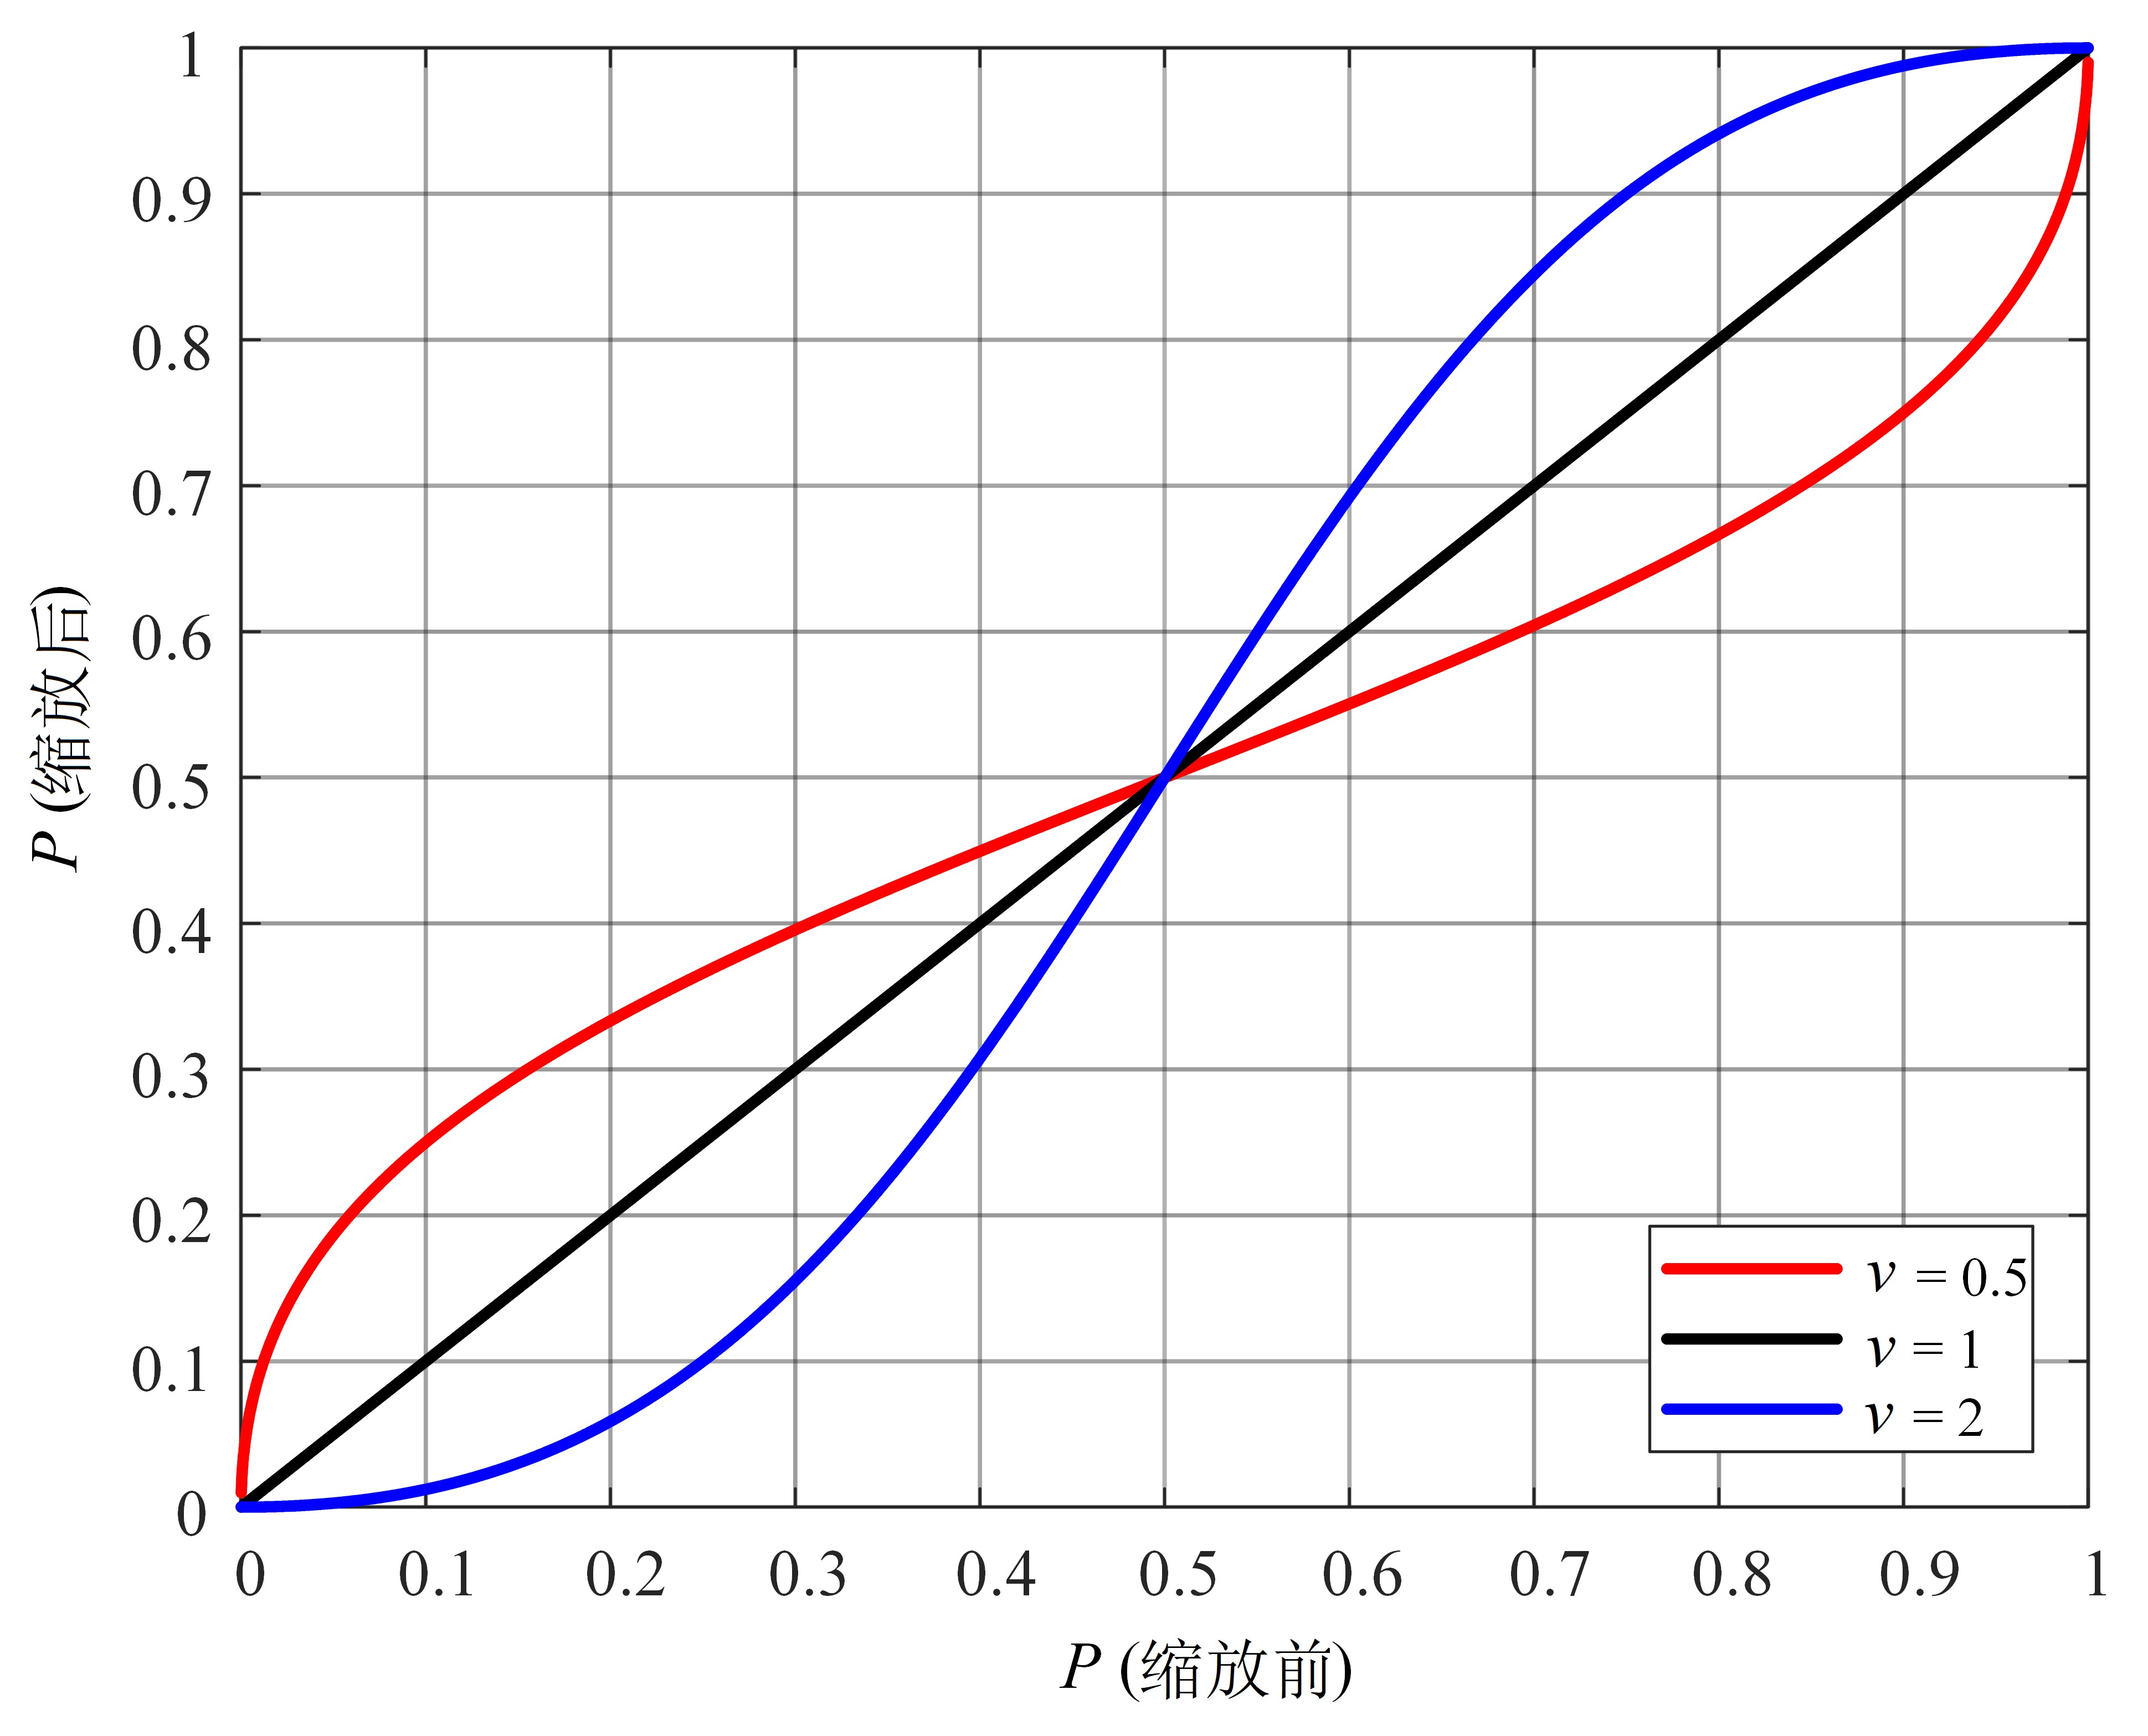
\includegraphics[width=10cm]{chapters/31}
	    \bicaption[\xiaosi 不同缩放系数v的缩放效果]{\wuhao 不同缩放系数v的缩放结果}{\wuhao Scaling results with different scaling coefficients ν}
	   	 \label{fig:3.1}
\end{figure}

%调整图片与下方文字之间的间距
%\vspace{-0.35cm}

图片标题与图片之间的间距使用默认设置即可,与上下文的间距由于LATEX动态排版特性,和该页的整体布局有关,需要大家手动调整。

。

。





下图是多子图示例,对于标题没有超过一行的图题,可以参照下面代码进行设置:
\vspace{0.5cm} %调整图片与上文的间距
\begin{figure}[!h]
	\centering
	\subfigure[]{
		\label{fig:666}
		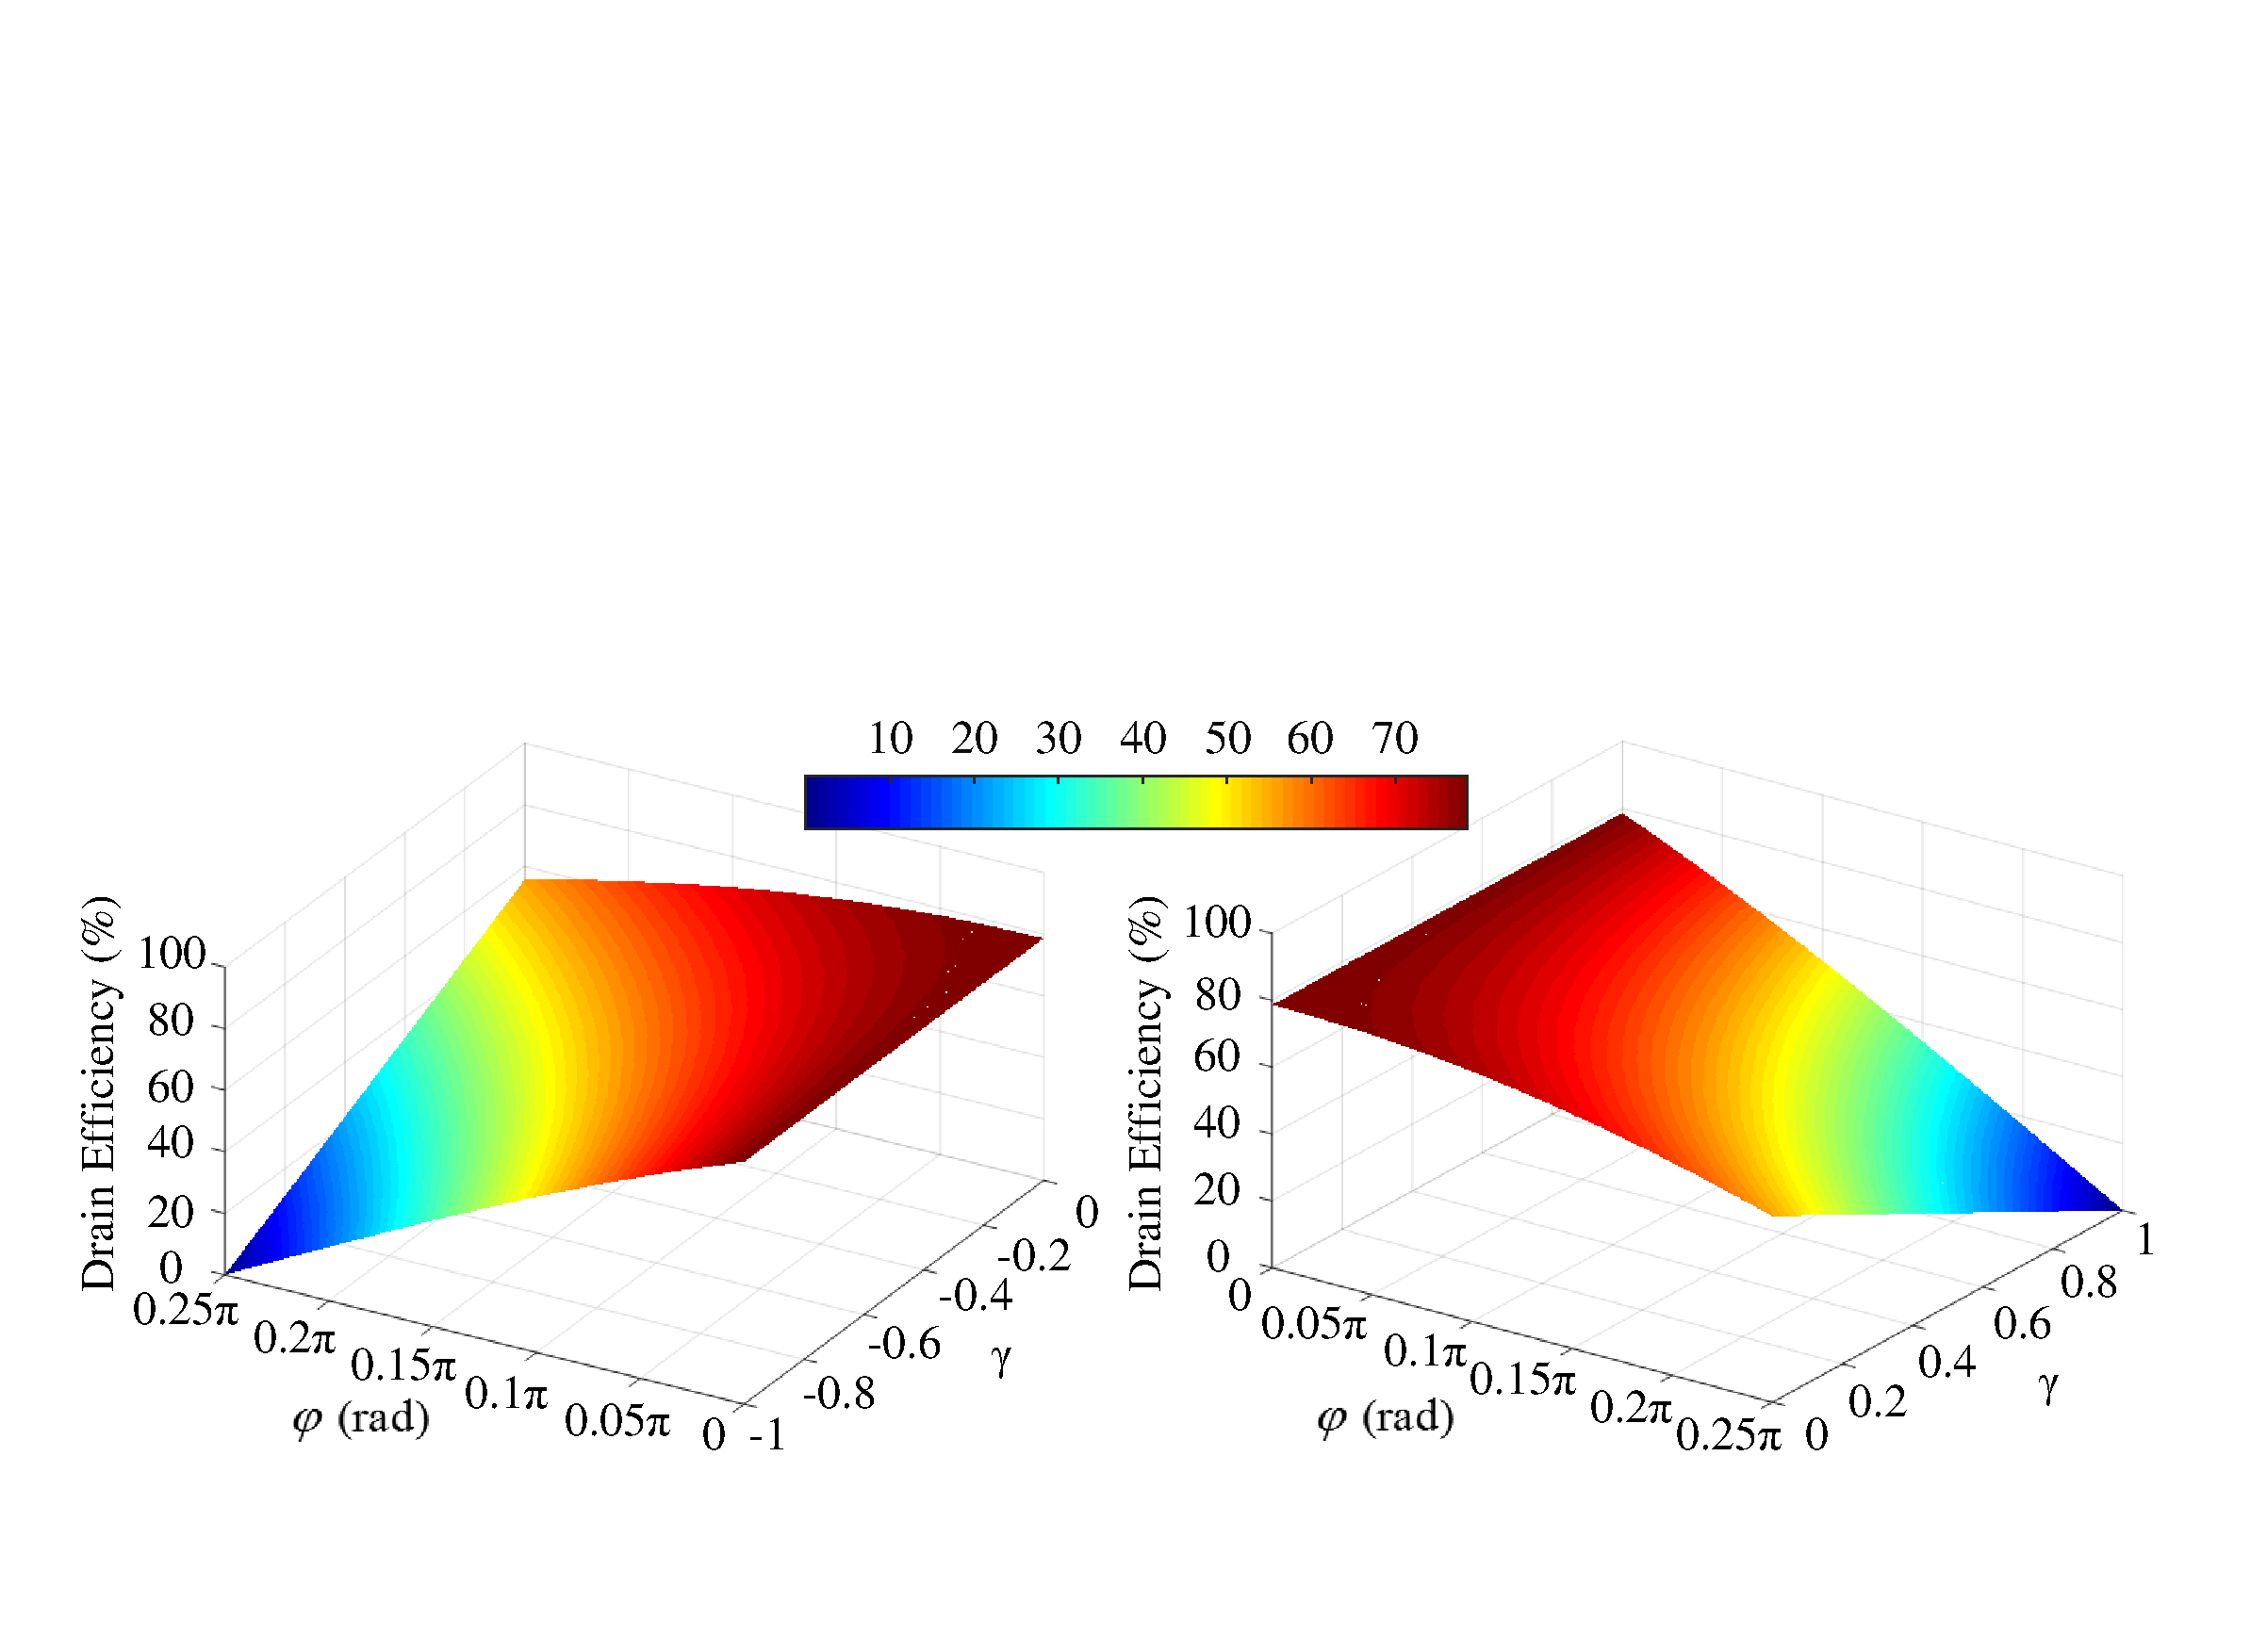
\includegraphics[width=12cm]{chapters/DE_J.pdf}}
	\subfigure[]{
		\label{fig:888}
		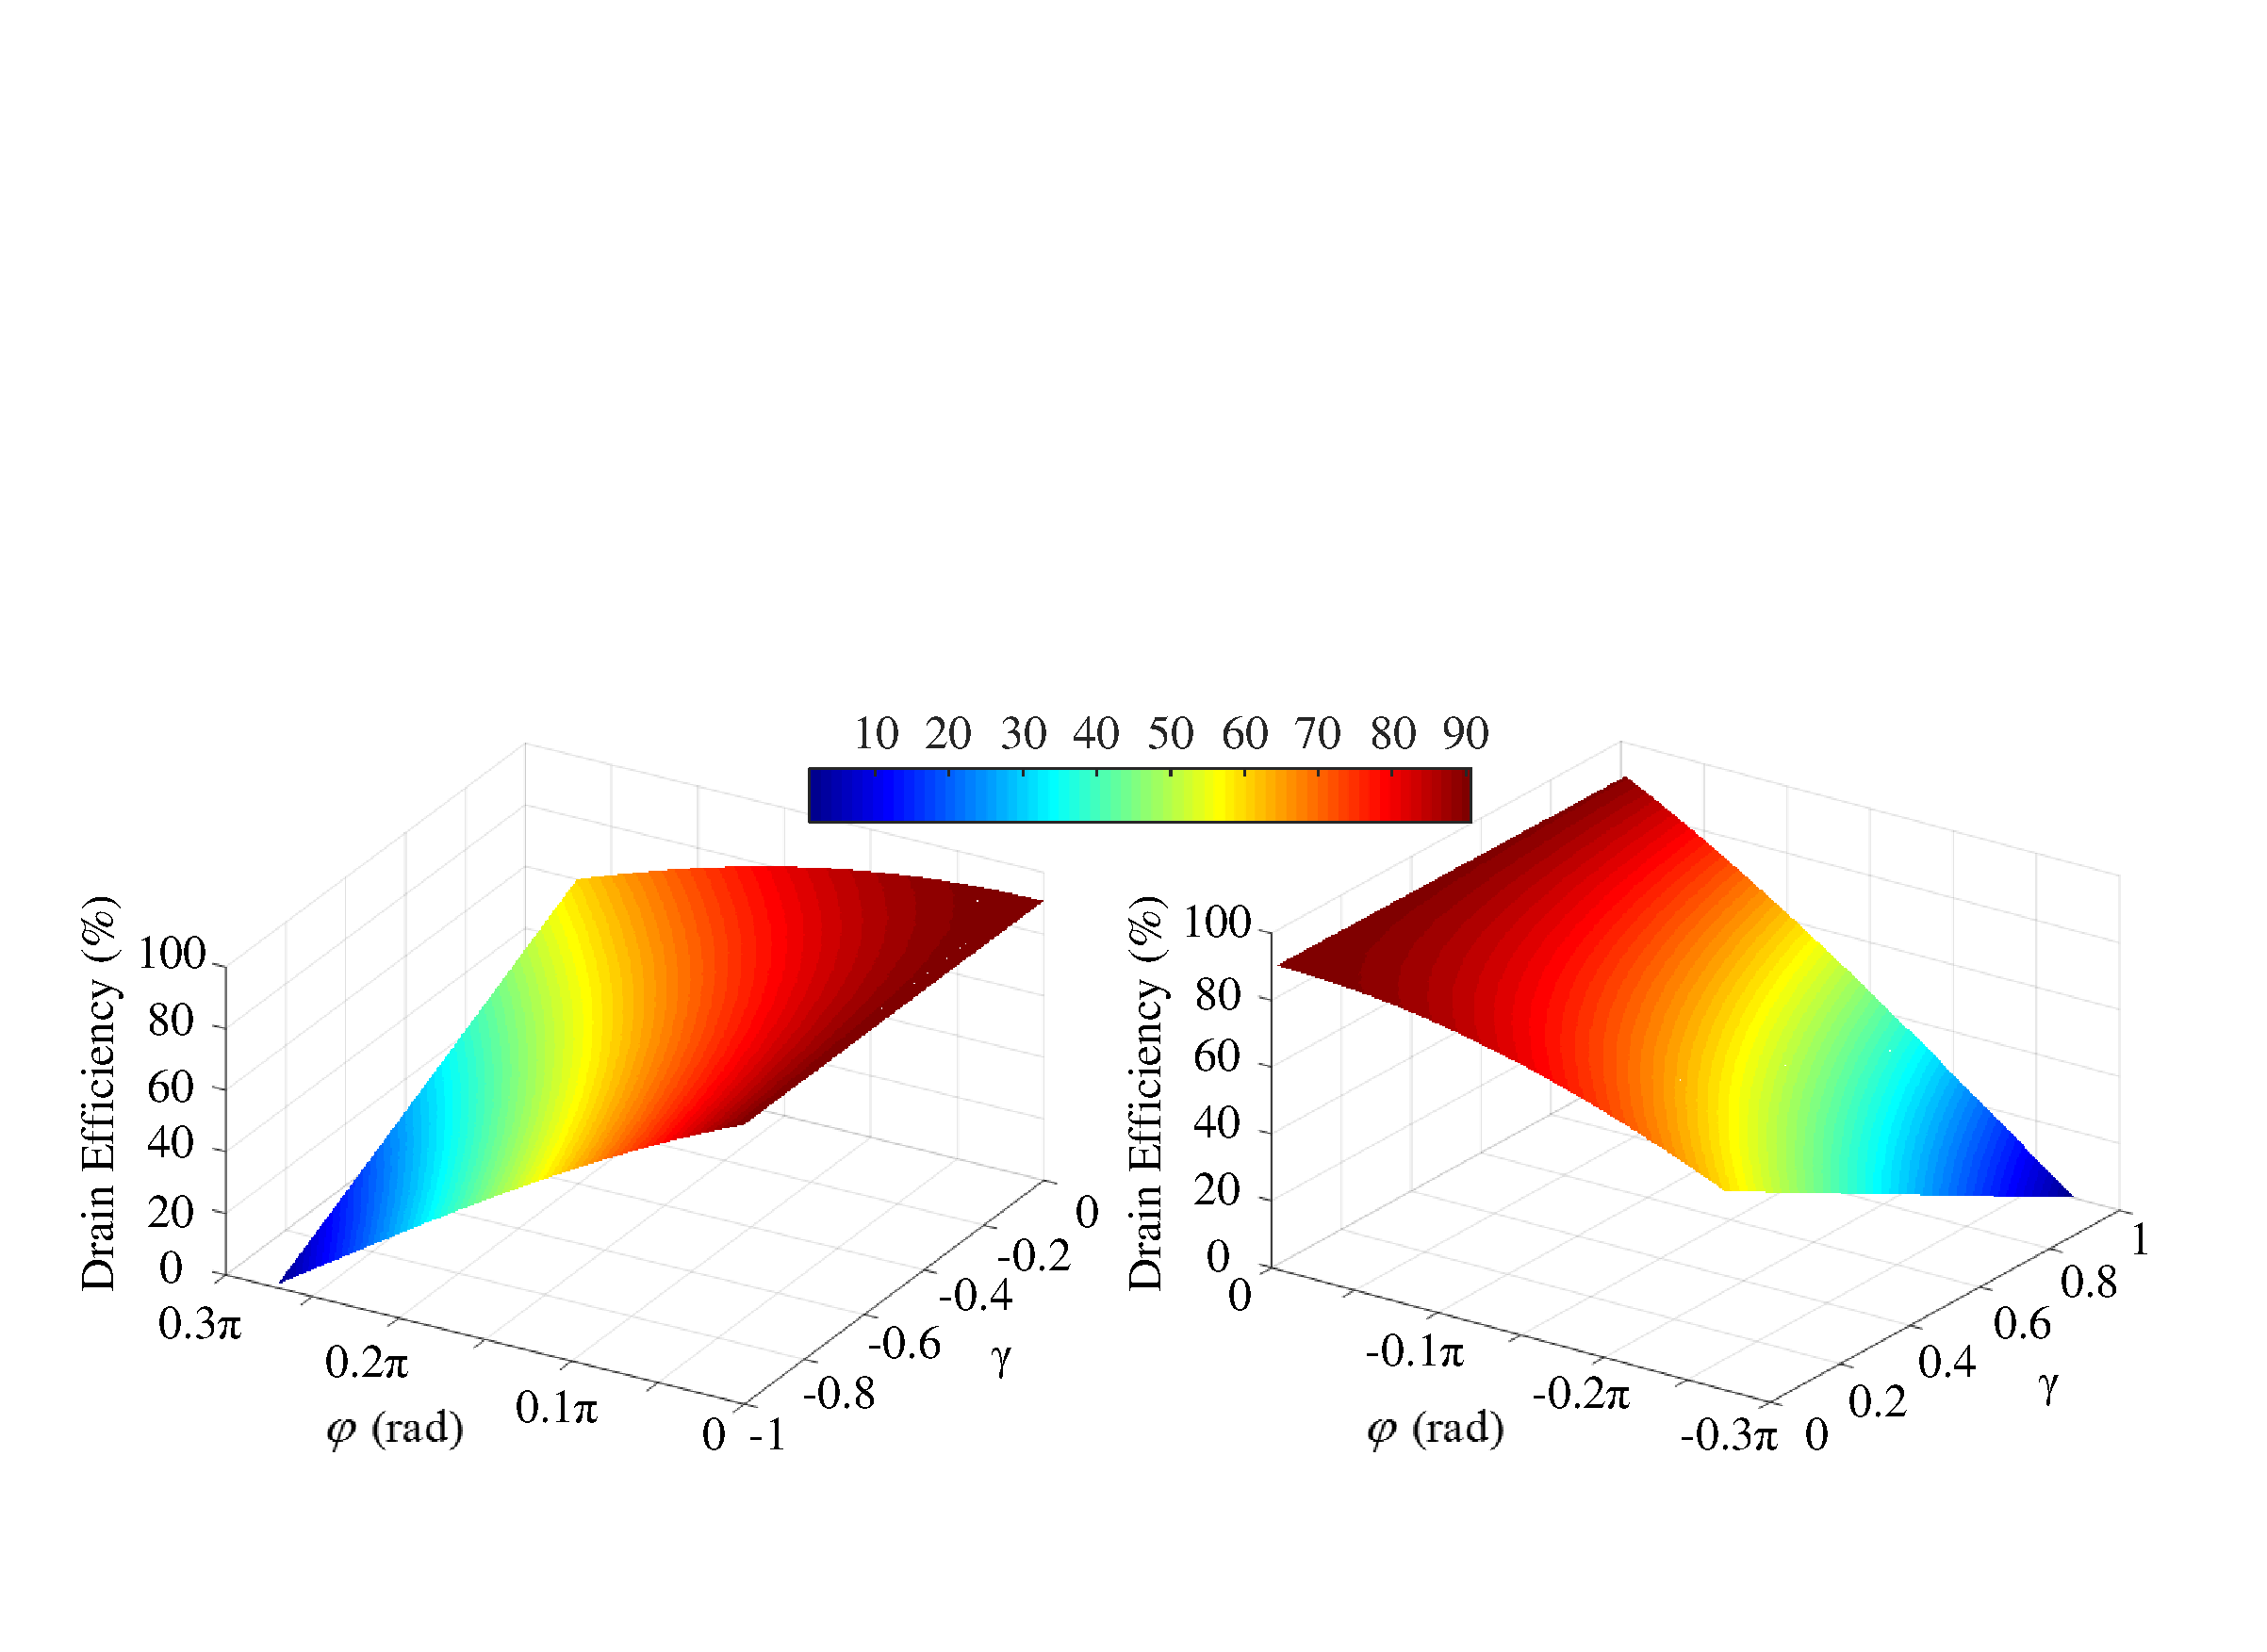
\includegraphics[width=12cm]{chapters/DE_CF.pdf}}
		\bicaption[\xiaosi 理论效率与$\gamma$和$\varphi$的关系]{\wuhao 理论效率与$\gamma$和$\varphi$的关系。 (a) $\alpha=1$; (b) $\alpha=2/\sqrt{3}$}{\wuhao Theoretical DE versus $\gamma$ and $\varphi$. (a) $\alpha=1$; (b) $\alpha=2/\sqrt{3}$}
\end{figure}
\vspace{-0.2cm} %调整图片与下文的间距
图片要求参照写作指南。图片要求参照写作指南。图片要求参照写作指南。图片要求参照写作指南。图片要求参照写作指南。图片要求参照写作指南。图片要求参照写作指南。图片要求参照写作指南。图片要求参照写作指南。图片要求参照写作指南。图片要求参照写作指南。图片要求参照写作指南。图片要求参照写作指南。图片要求参照写作指南。
图片要求参照写作指南。图片要求参照写作指南。图片要求参照写作指南。图片要求参照写作指南。图片要求参照写作指南。图片要求参照写作指南。图片要求参照写作指南。图片要求参照写作指南。图片要求参照写作指南。图片要求参照写作指南。图片要求参照写作指南。图片要求参照写作指南。图片要求参照写作指南。图片要求参照写作指南。图片要求参照写作指南。图片要求参照写作指南。图片要求参照写作指南。图片要求参照写作指南。图片要求参照写作指南。图片要求参照写作指南。图片要求参照写作指南。


对于图题超过了一行的图片,请参照下面代码进行设置,使得图题能与WORD一样居中左对齐,注意其中bicaption[]()(这个里面的字号使用wuhaob):
\vspace{0.3cm}
\begin{figure}[!h]
	\centering
	\subfigure[]{
		\label{fig:DE_J}
		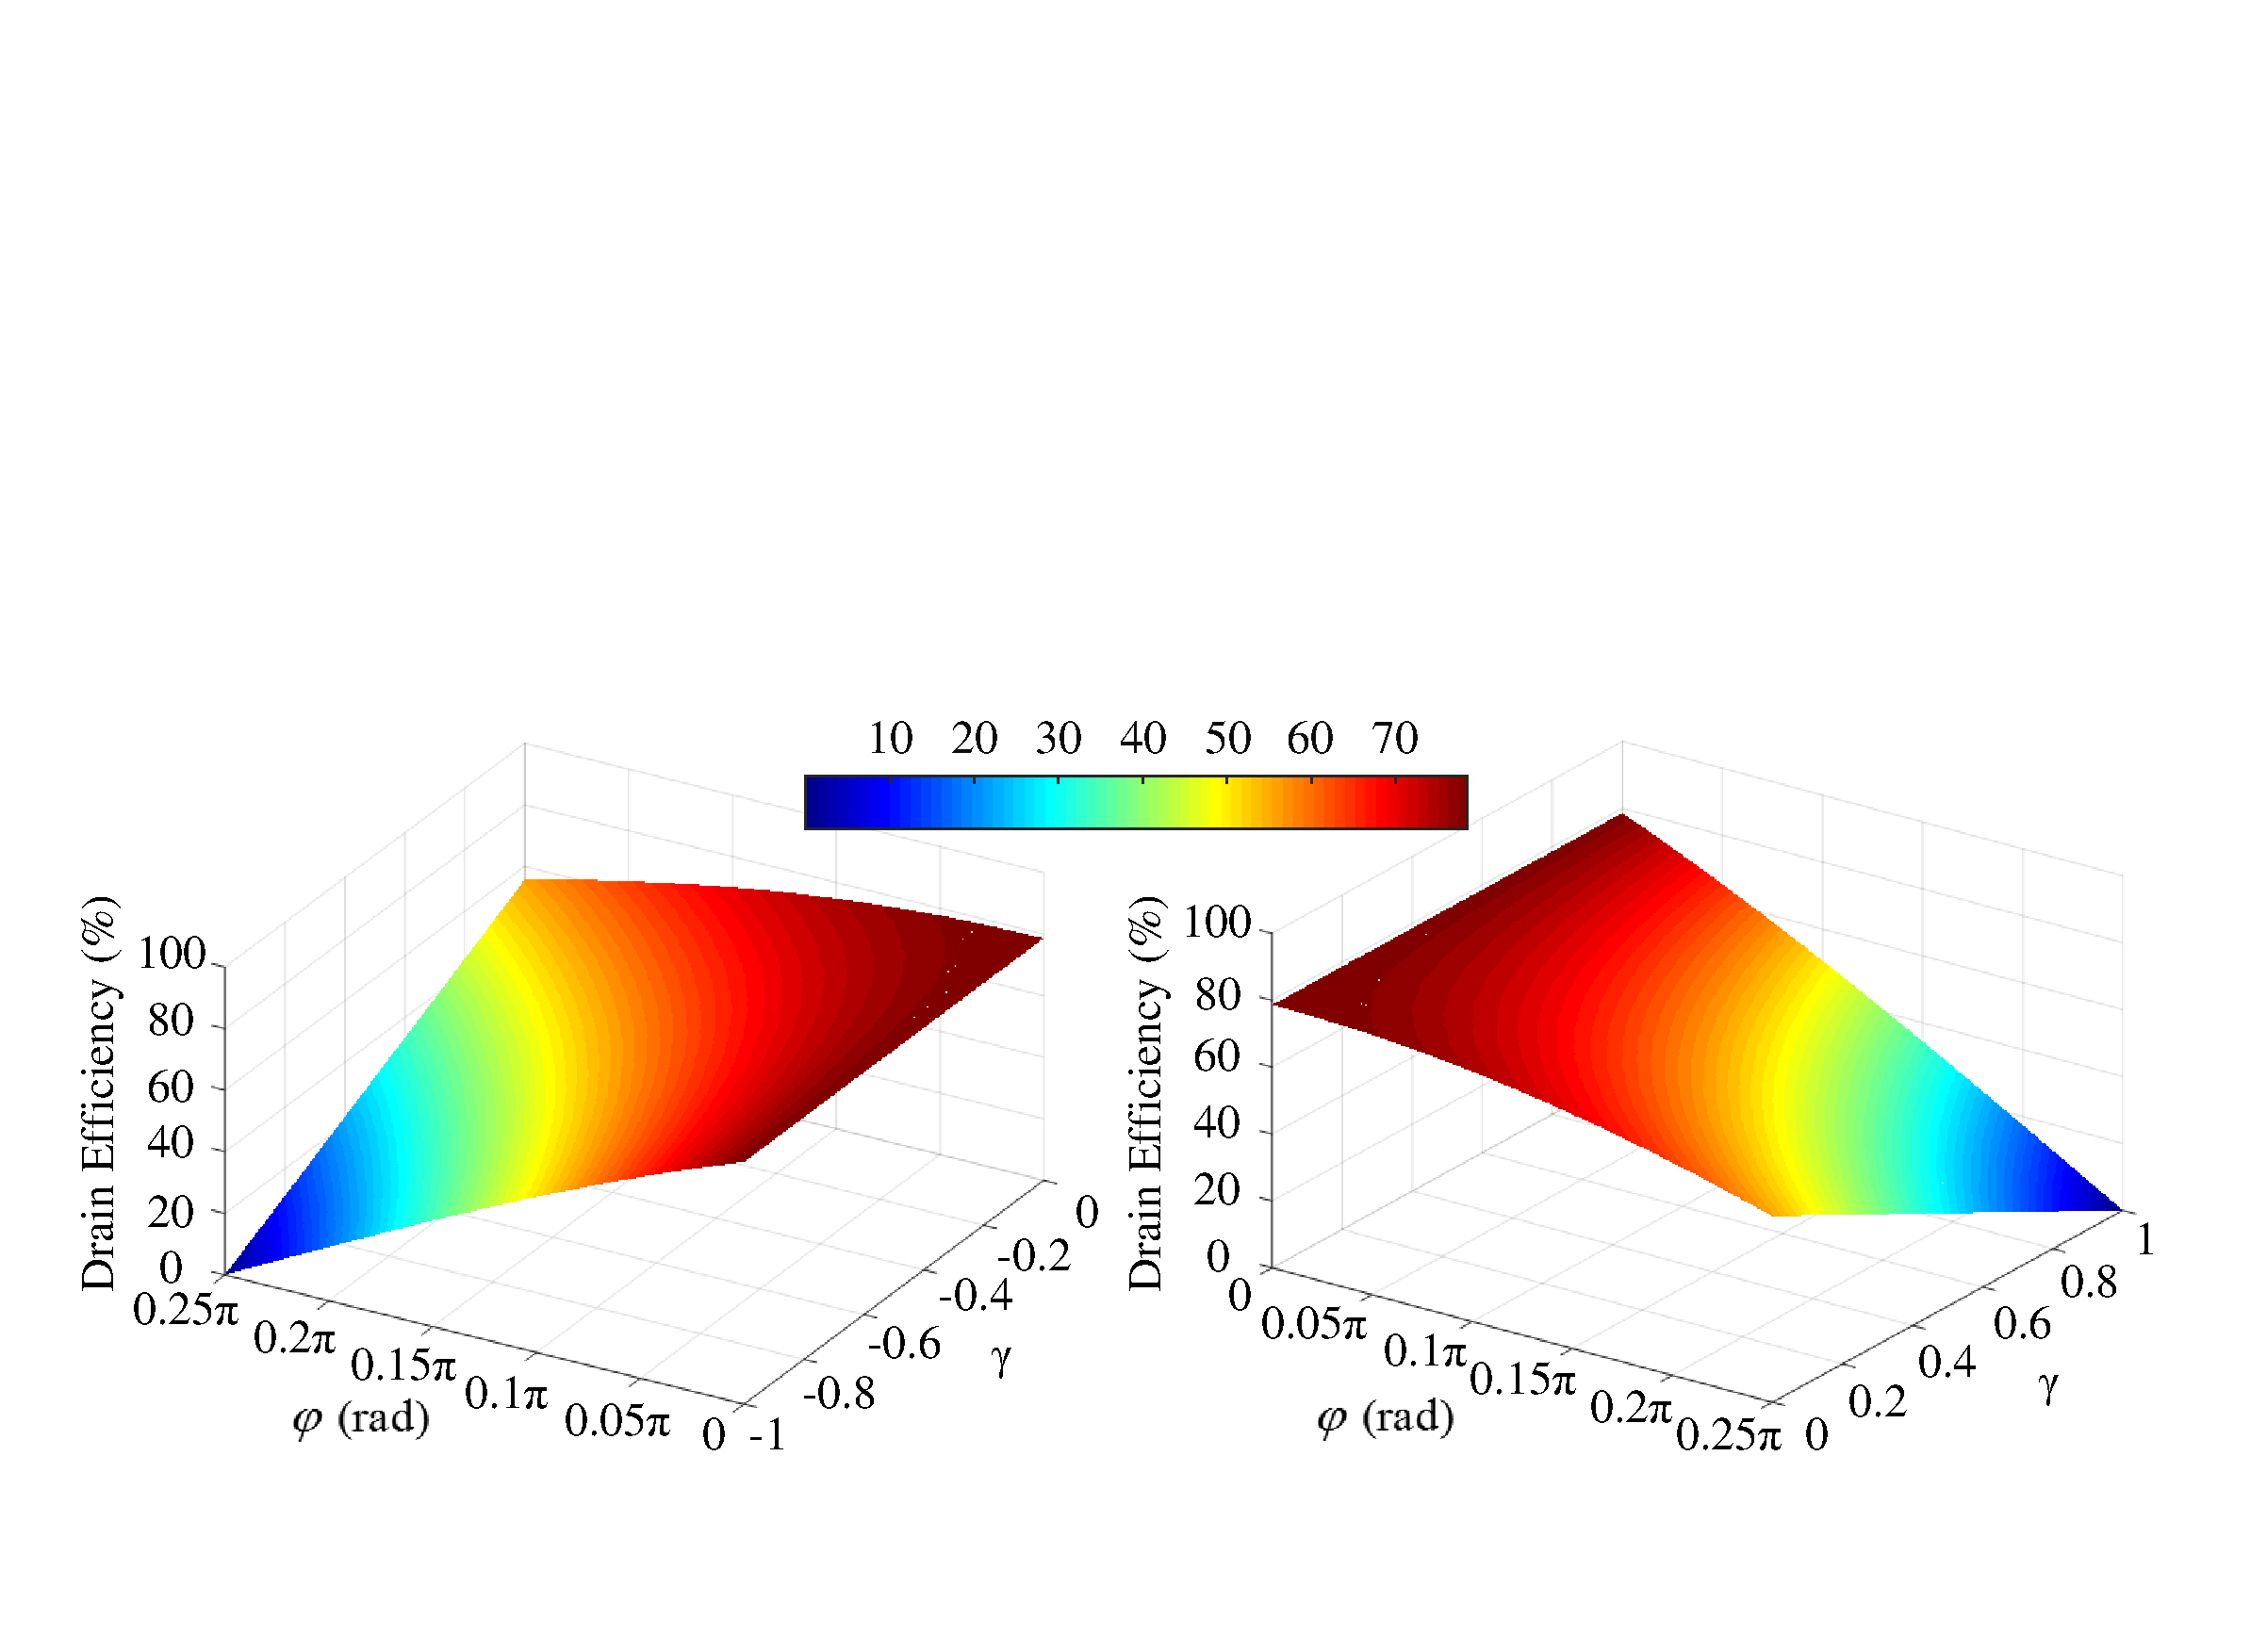
\includegraphics[width=12cm]{chapters/DE_J.pdf}}
	\subfigure[]{
		\label{fig:DE_CF}
		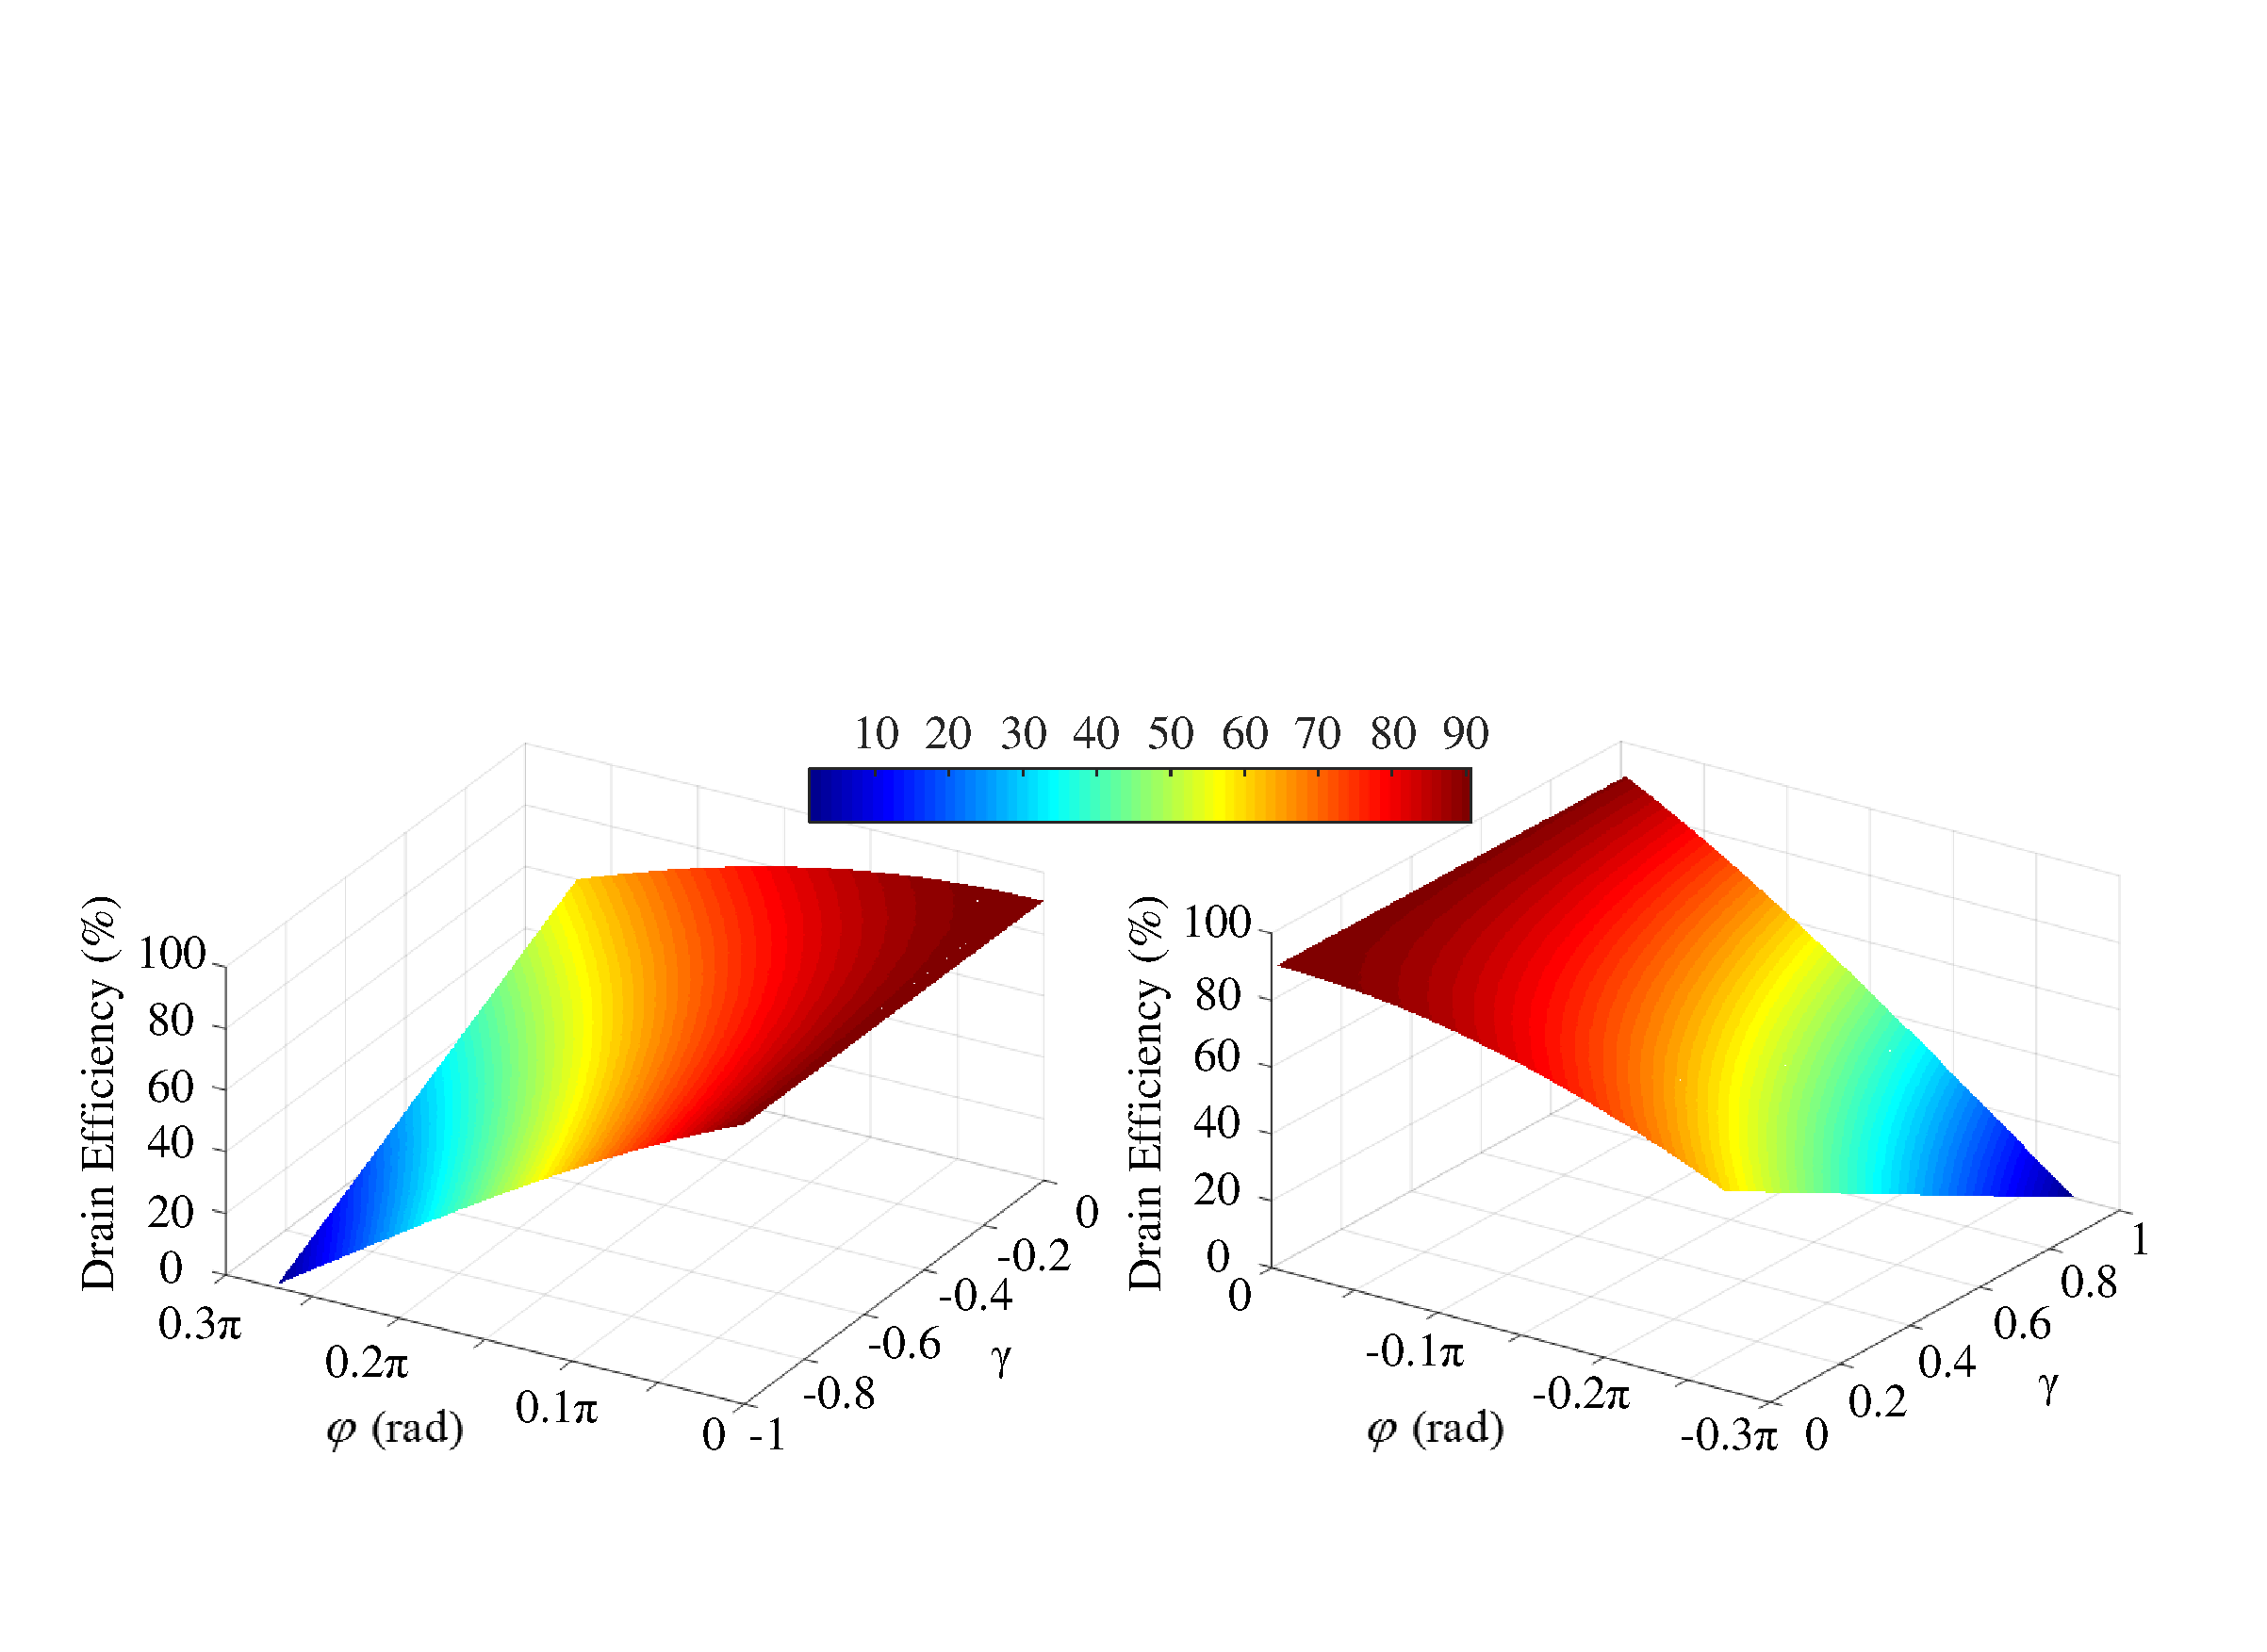
\includegraphics[width=12cm]{chapters/DE_CF.pdf}}
	\begin{itemize}[leftmargin=1.6cm,rightmargin=1.6cm]
		\item[\quad] \bicaption[\xiaosi 理论效率与$\gamma$和$\varphi$的关系]
		{\wuhao 理论效率与$\gamma$和$\varphi$的关系。 (a) $\alpha=1$; (b) $\alpha=2/\sqrt{3}$}
		{\wuhaob Theoretical DE versus $\gamma$ and $\varphi$. (a) $\alpha=1$; (b) $\alpha=2/\sqrt{3}$Theoretical DE versus $\gamma$ and $\varphi$. (a) $\alpha=1$; (b) $\alpha=2/\sqrt{3}$}
	\end{itemize}
\vspace{-1cm}


%\captionsetup{margin={1.6cm,1.6cm}}
%\bicaption[\xiaosi 理论效率与$\gamma$和$\varphi$的关系。]{\wuhao 理论效率与$\gamma$和$\varphi$的关系。 (a) $\alpha=1$; (b) $\alpha=2/\sqrt{3}$}{\wuhaob Theoretical DE versus $\gamma$ and $\varphi$. (a) $\alpha=1$; (b) $\alpha=2/\sqrt{3}$Theoretical DE versus $\gamma$ and $\varphi$. (a) $\alpha=1$; (b) $\alpha=2/\sqrt{3}$}


\end{figure}



\subsection{表}
% \vspace{0.1cm}  % 添加0.1厘米的垂直空间
% 
% \begin{table}[h]  % 开始表格环境,h表示尽量将表格放在当前位置
% 	\renewcommand{\arraystretch}{1.5}  % 设置表格行距为1.5倍
% 	\centering  % 表格居中
% 	\bicaption[\xiaosi 电流类型对效率的影响]{\wuhao 电流类型对效率的影响}{\wuhao Current type impact on efficiency}  % 双语标题,方括号内是目录中显示的标题(小四号字),第一个花括号内是中文标题(五号字),第二个花括号内是英文标题(五号字)
% 	\begin{tabular}{p{3cm}p{3cm}p{3cm}p{3cm}}  % 开始表格内容,定义4列,每列宽度为3厘米,p表示允许文本自动换行
% 		\toprule[1.5pt]  % 顶部粗线,粗细为1.5pt
% 		\makecell[c]{\songti\wuhao 电流类型}&\makecell[c]{\songti\wuhao A}&\makecell[c]{\songti\wuhao B}&\makecell[c]{\songti\wuhao C}\\  % 表头行,\makecell[c]表示单元格内容居中,\songti表示宋体,\wuhao表示五号字
% 		\hline  % 普通横线
% 		\makecell[c]{\wuhao aaa}&\makecell[c]{\wuhao aa1}&\makecell[c]{\wuhao bb1}&\makecell[c]{\wuhao cc1}\\  % 数据行,格式同上
% 		\bottomrule[1.5pt]  % 底部粗线,粗细为1.5pt
% 	\end{tabular}
%    \label{tab:3.1}  % 表格标签,用于交叉引用	
% \end{table}
%
% \vspace{-0.1cm}  % 调整表格与下文的间距
表格格式参照写作指南。表格格式参照写作指南。表格格式参照写作指南。表格格式参照写作指南。表格格式参照写作指南。表格格式参照写作指南。表格格式参照写作指南。表格格式参照写作指南。表格格式参照写作指南。表格格式参照写作指南。表格格式参照写作指南。表格格式参照写作指南。表格格式参照写作指南。表格格式参照写作指南。表格格式参照写作指南。表格格式参照写作指南。

\vspace{-0.1cm}

\begin{table*}[h]
	\renewcommand{\arraystretch}{1.5}
	\bicaption[\xiaosi 高效率功放性能对比]{\wuhao 高效率功放性能对比}{\wuhao High-effiency power amplifier performance comparison}
	\label{tab_1}
	\centering
	\wuhao
	\begin{tabular}{c c c c c }
		\hline
		{\textbf{带宽}(GHz)}&{\textbf{功率}(dBm)}&{\textbf{效率}(\%)}&{\textbf{线性度}(dBc)}&{\textbf{信号带宽}(MHz)}\\
		\hline
		1.4--2.6&32--34&30--40 (DE)&-25 -- -30 (ACLR)&5\\
		\hline
		\multirow{2}{*}{2.1--2.7}&39&45 (DE) @ 2.14 GHz&--31 (ACLR)&\multirow{2}{*}{\diagbox{\qquad}{\qquad}}\\\cline{3-4}
		&(average)&40 (DE) @ 2.655 GHz&--30 (ACLR)& \\
		\hline
		3.5&38.1&59 (PAE)&30 (C/I)&5\\
		\hline
		\multirow{2}{*}{1.6--2.6}&36.0--38.5&45--60 (PAE)&30 (C/I)&5\\\cline{2-5}
		&35.3--37.5&40--55 (PAE)&--30 (ACLR)&20\\
		\hline
	\end{tabular}
\end{table*}

算法表示例:XXXXXXXX,如算法3-1所示。

\begin{table}[!htb]
	\setlength{\belowcaptionskip}{6pt}
	\setlength{\abovecaptionskip}{6pt}
	\centering
	%	\caption{\wuhao DQN算法训练过程}
	%	{\wuhao Table2-1 Training process of DQN\\[6pt]}
	\renewcommand{\arraystretch}{1.2}
	\begin{tabular}{p{13.2cm}}
		\toprule[1.5pt]
		\makecell[l]{\songti\wuhao 算法3-1 XXXXXX训练过程}\\
		\midrule[0.75pt]
		\makecell[l]{\wuhao 1: \ \ xxxxxx缓存$D$以及xxxxxx量为$\theta$的xxxxx络;}\\
		\makecell[l]{\wuhao 2: \ \ \textbf{for} episodes $=0, 1,\cdots ,E$ \textbf{do}}\\
		\makecell[l]{\wuhao 3: \quad \ \ 初始xxxxx向量$\Phi (s)$并将其作为xxxxxxxx值;}\\
		\makecell[l]{\wuhao 4: \quad \ \ \textbf{for} $t =0, 1,\cdots ,T$ \textbf{do}}\\
		\makecell[l]{\wuhao 5: \qquad \ \ 以xxx率$\epsilon$选xxxxx动作$a$;}\\
		\makecell[l]{\wuhao 6: \qquad \ \ 否xxx动作${{a}}={{\max }_{\hat{a}}}Q(\Phi ({{s}}),\hat{a}|\theta )$;}\\
		\makecell[l]{\wuhao 6: \qquad \ \ 执xxx动作$a$并观xxx奖励$r$和下一状态$s^{\prime }$;}\\
		\makecell[l]{\wuhao 7: \qquad \ \ 将经验$(\Phi ({{s}}),a,r,\Phi ({s^{\prime }}))$存储xxxx缓存$D$;}\\
		\makecell[l]{\wuhao 8: \qquad \ \ 从$D$中XXXX择$c$个样本$(\Phi ({{s_j}}),a_j,r_j,\Phi ({{s_j}^{\prime }}))$,并XXXXXXX计算$y_j$;
		}\\
		\makecell[l]{\wuhao 9: \qquad \ \ 根据xxxxx差;}\\
		\makecell[l]{\wuhao 10: \qquad xxxxxxx下降法更新$\theta$;}\\
		\makecell[l]{\wuhao 11: \quad \textbf{end for}}\\
		\makecell[l]{\wuhao 12: \textbf{end for}}\\
		\bottomrule[1.5pt]
	\end{tabular}
	\label{tab:2.1} 
\end{table}


% \begin{table}[!htb]  % 创建表格环境,!htb表示优先放在当前位置(here),其次顶部(top),再次底部(bottom)
%     \setlength{\belowcaptionskip}{6pt}  % 设置标题下方间距为6pt
%     \setlength{\abovecaptionskip}{6pt}  % 设置标题上方间距为6pt
%     \centering  % 表格居中
%     %	\caption{\wuhao DQN算法训练过程}  % 被注释掉的中文标题
%     %	{\wuhao Table2-1 Training process of DQN\\[6pt]}  % 被注释掉的英文标题
%     \renewcommand{\arraystretch}{1.2}  % 设置行间距为1.2倍
%     \begin{tabular}{p{13.2cm}}  % 创建表格,p{13.2cm}表示单列表格,列宽为13.2厘米,可自动换行
%         \toprule[1.5pt]  % 顶部粗线,粗细为1.5pt
%         \makecell[l]{\songti\wuhao 算法3-1 XXXXXX训练过程}\\  % 左对齐的表格单元格,使用宋体五号字体
%         \midrule[0.75pt]  % 中部细线,粗细为0.75pt
%         \makecell[l]{\wuhao 1: \ \ xxxxxx缓存$D$以及xxxxxx量为$\theta$的xxxxx络;}\\  % 算法第1行
%         \makecell[l]{\wuhao 2: \ \ \textbf{for} episodes $=0, 1,\cdots ,E$ \textbf{do}}\\  % 算法第2行,for循环加粗
%         \makecell[l]{\wuhao 3: \quad \ \ 初始xxxxx向量$\Phi (s)$并将其作为xxxxxxxx值;}\\  % 算法第3行,缩进
%         \makecell[l]{\wuhao 4: \quad \ \ \textbf{for} $t =0, 1,\cdots ,T$ \textbf{do}}\\  % 算法第4行,嵌套for循环
%         \makecell[l]{\wuhao 5: \qquad \ \ 以xxx率$\epsilon$选xxxxx动作$a$;}\\  % 算法第5行,更多缩进
%         \makecell[l]{\wuhao 6: \qquad \ \ 否xxx动作${{a}}={{\max }_{\hat{a}}}Q(\Phi ({{s}}),\hat{a}|\theta )$;}\\  % 算法第6行
%         \makecell[l]{\wuhao 6: \qquad \ \ 执xxx动作$a$并观xxx奖励$r$和下一状态$s^{\prime }$;}\\  % 算法第6行(重复的行号)
%         \makecell[l]{\wuhao 7: \qquad \ \ 将经验$(\Phi ({{s}}),a,r,\Phi ({s^{\prime }}))$存储xxxx缓存$D$;}\\  % 算法第7行
%         \makecell[l]{\wuhao 8: \qquad \ \ 从$D$中XXXX择$c$个样本$(\Phi ({{s_j}}),a_j,r_j,\Phi ({{s_j}^{\prime }}))$,并XXXXXXX计算$y_j$;
%         }\\  % 算法第8行,包含数学公式
%         \makecell[l]{\wuhao 9: \qquad \ \ 根据xxxxx差;}\\  % 算法第9行
%         \makecell[l]{\wuhao 10: \qquad xxxxxxx下降法更新$\theta$;}\\  % 算法第10行
%         \makecell[l]{\wuhao 11: \quad \textbf{end for}}\\  % 算法第11行,内层循环结束
%         \makecell[l]{\wuhao 12: \textbf{end for}}\\  % 算法第12行,外层循环结束
%         \bottomrule[1.5pt]  % 底部粗线,粗细为1.5pt
%     \end{tabular}
%     \label{tab:2.1}  % 表格标签,可通过\ref{tab:2.1}引用
% \end{table}



\section{公式格式}

\begin{equation}
\left\{ \begin{aligned}
0.794 \le \zeta  \le 1 ~~~~~~~~~~~\\
0.631 \le \gamma  = \frac{{0.631}}{{{\zeta ^2}}} \le 1~~~~~~ \\
- \frac{1}{{2\gamma }} \le \delta  \le \frac{1}{{2\gamma }}~~~~~~~~~~~ \\
{Z_{c,low,f}} = 2{R_{opt}}(\gamma  + j\delta )~~~~~\\
{Z_{c,2f}} = {Z_{c,low,2f}} =  - j\frac{{3\pi }}{4}\gamma \delta {R_{opt}}
\end{aligned} \right.
\label{eq:3.1}
\end{equation}

\begin{equation}
\begin{aligned}
v(\theta ) = V_{DD}\cdot(1 - \alpha cos(\theta  + \varphi ) + \beta cos(3\theta  + 3\varphi ))\\
\cdot(1 - \gamma \sin (\theta  + \varphi )) ~~~~~- 1 \le \gamma  \le 1\
\end{aligned}
\label{eq:vd}
\end{equation}

\begin{equation}
\begin{aligned}
att\left( {{\bm{q}},{\bm{k}},{\bm{v}}} \right) = softmax\left( {\frac{{{\bm{qk}}^{\rm T} }}
	{{\sqrt {d_{\bm{k}} } }}} \right){\bm{v}}
\end{aligned}
\label{eq:2.12}
\end{equation}





\noindent
公式格式测试。${\mathbf{\Theta }} = \left\{ {{\theta _k}\left( n \right),\forall k,n} \right\}$

\section{印制要求}
涉密学位论文的印刷、制作、传递、存档等,须符合国家、学校相关保密要求。学位论文一律左侧装订。

中文摘要之前的前置部分(封面、中、英文题名页、独创性声明和使用授权书),采用单面印刷。

从中文摘要开始,采用双面印刷。

中文摘要及之后的前置部分,包括中文摘要、ABSTRACT、目录、图目录(如有)、表目录(如有)、主要符号表(如有)、缩略词表(如有),在双面印刷时,若某部分页数为奇数,则该部分最后一页单面印刷。例如:若“摘要”只有1页,则其页码是“Ⅰ”,第“Ⅰ”页纸的背面为空白(无页眉或页码);“ABSTRACT”用新的一张纸印刷,页码从“Ⅱ”开始。

从第1章第1页开始,至论文最后1页,所有页面均双面印刷。例如:若第1章的最后1页为第17页,则第2章的第1页在第17页的背面印刷,页码为“18”(页眉是“重庆邮电大学博士(硕士)学位论文”)。

一次性双面打印整本学位论文技巧:除用于打印的版本外,电子版论文中一律不得出现空白页。论文打印建议使用PDF格式。为方便一次性双面打印,有时可在单面印刷的部分(如封面、中、英文题名页、独创性声明和使用授权书),或者双面打印只有1页的某部分内容(如摘要、ABSTRACT等)后插入1页空白页,该空白页不编排页眉页码;论文中出现的页码应前后连续,不得中断。


\section{本章小结}
本章介绍了……



\begin{table}[!htb]
	\setlength{\belowcaptionskip}{6pt}
	\setlength{\abovecaptionskip}{6pt}
	\centering
	\renewcommand{\arraystretch}{1.2}
	\begin{tabular}{p{13.2cm}}
		\toprule[1.5pt]
		\makecell[l]{\songti\wuhao 算法3-1 VFPU 算法训练过程}\\
		\midrule[0.75pt]
		\makecell[l]{\wuhao \textbf{Input:} Parties $B,C$. Aligned datasets ${{\mathsf{\mathcal{D}}}_{B}}\text{,}{{\mathsf{\mathcal{D}}}_{C}}$ and ID sets ${{\mathsf{\mathcal{I}}}_{B}}\text{,}\ {{\mathsf{\mathcal{I}}}_{C}}$. Maximum}\\
		\makecell[l]{\wuhao \quad number of iterations $M$, number of random sampling iterations $T$ and $\theta$ where $\theta$ is the}\\
		\makecell[l]{\wuhao \quad sampling rate of reliable positive samples.}\\
		\makecell[l]{\wuhao \textbf{Output:} $R$, a set of reliable positive samples.}\\
		\makecell[l]{\wuhao \textbf{Party C executes:}}\\
		\makecell[l]{\wuhao 1: \ \ \textbf{for} $m=1,2,\ldots,M$ \textbf{do}}\\
		\makecell[l]{\wuhao 2: \quad \ \ ${{P}_{m}}=\{i|\mathsf{\mathcal{Y}}_{i}^{C}=1, \ i\in {{\mathsf{\mathcal{I}}}_{C}}\}$}\\
		\makecell[l]{\wuhao 3: \quad \ \ ${{U}_{m}}=\{i|\mathsf{\mathcal{Y}}_{i}^{C}=-1, \ i\in {{\mathsf{\mathcal{I}}}_{C}}\}$}\\
		\makecell[l]{\wuhao 4: \quad \ \ \textbf{for} $t=1,2,\ldots,T$ \textbf{do}}\\
		\makecell[l]{\wuhao 5: \qquad \ \ $N_{m}^{t}=\{Randomly\ select\ |{{P}_{m}}|\ elements\ from\ {{U}_{m}} \}$}\\
		\makecell[l]{\wuhao 6: \qquad \ \ $O_{m}^{t}={{U}_{m}}-N_{m}^{t}$}\\
		\makecell[l]{\wuhao 7: \qquad \ \ Encrypt and send $N_{m}^{t}$, ${P_m}$, and $O_{m}^{t}$ to other parties.}\\
		\makecell[l]{\wuhao 8: \qquad \ \ Notify parties to set training data and testing data.}\\
		\makecell[l]{\wuhao 9: \qquad \ \ $S_m^t$ = Base\_Estimator\_Learning()}\\
		\makecell[l]{\wuhao 10: \quad \textbf{end for}}\\
		\makecell[l]{\wuhao 11: \quad ${{\mathsf{\mathcal{P}}}_{m}}(u)={\sum\nolimits_{t=1}^{T}{S_{m}^{t}}}(u)/{\sum\nolimits_{t=1}^{T}{I(u\in O_{m}^{t})\text{,}\ \ \forall \text{u}\in }}\;{{U}_{m}}$}\\
		\makecell[l]{\wuhao 12: \quad ${{R}_{m}}=\{Chose\ Top\ |{{U}_{m}}|\times \theta \ IDs\ from\ {{\mathsf{\mathcal{P}}}_{m}}\}$}\\
		\makecell[l]{\wuhao 13: \quad $\mathsf{\mathcal{Y}}_{r}^{C}=1\text{,}\ \ \forall r\in {{R}_{m}}$}\\
		\makecell[l]{\wuhao 14: \textbf{end for}}\\
		\makecell[l]{\wuhao 15: $R=\bigcup\limits_{m=1}^{M}{{{R}_{m}}}$}\\
		\makecell[l]{\wuhao \textbf{Function} Base\_Estimator\_Learning():}\\
		\makecell[l]{\wuhao 16: \quad Server creates encryption pairs, sends public keys to $B$ \& $C$}\\
		\makecell[l]{\wuhao 17: \quad $B$ \& $C$ encrypt, exchange gradients \& losses.}\\
		\makecell[l]{\wuhao 18: \quad $B$ \& $C$ add masks, send encrypted values to server.}\\
		\makecell[l]{\wuhao 19: \quad Server decrypts, sends back values. $B$ \& $C$ unmask, update models.}\\
		\makecell[l]{\wuhao 20: \quad \textbf{return} Predicted probabilities of positive class on testing data.}\\
		\bottomrule[1.5pt]
	\end{tabular}
	\label{tab:algo-vfpu} 
\end{table}